\chapter{Spécification des besoins}

\section{Introduction}

Le chapitre précédent a présenté le cadre général du projet au sein de Smart-Conseil,
l'analyse des solutions existantes face au harcèlement scolaire et leurs limites,
ainsi que la solution envisagée composée de quatre modules intelligents.

Ce chapitre définit ce que chaque module doit accomplir.
Il est organisé en cinq parties : les fonctionnalités attendues (besoins fonctionnels),
les contraintes de qualité (besoins non fonctionnels), les acteurs du système,
le diagramme de cas d'utilisation, et l'environnement technique retenu.

% ─────────────────────────────────────────────────────────────────────────────
\section{Identification des besoins fonctionnels}

Les besoins fonctionnels décrivent l'ensemble des fonctionnalités que le système doit
offrir à ses utilisateurs. Ils sont organisés par module.

% ── Module 1 : Noa ────────────────────────────────────────────────────────────
\subsection{Module 1 — Noa : assistant virtuel du site public}

Noa est l'assistant virtuel intégré au site public de Netethic.
Il aide les visiteurs à s'informer sur la plateforme et à planifier une démonstration.
Le Tableau~\ref{tab:bf_noa} présente ses besoins fonctionnels.

\vspace{6pt}
\begin{table}[H]
\caption{Besoins fonctionnels — Noa (assistant site public Netethic)}
\label{tab:bf_noa}
\centering
\small
\setlength{\tabcolsep}{4pt}
\begin{tabular}{|c|p{3.5cm}|p{9.5cm}|}
\hline
\textbf{ID} & \textbf{Besoin} & \textbf{Description} \\
\hline
BF-N01 & Répondre aux questions
        & L'assistant répond aux questions des visiteurs sur les fonctionnalités, les tarifs, le RGPD et les coordonnées de Netethic. \\
\hline
BF-N02 & Gérer la conversation et mémoriser les réponses
        & Le système conserve l'historique des échanges pour maintenir la cohérence de la conversation et retourne instantanément les réponses déjà calculées. \\
\hline
BF-N03 & Classifier l'intention
        & Chaque message est analysé selon son intention — bavardage, question, suivi ou requête interdite — pour lui appliquer le traitement adapté. \\
\hline
BF-N05 & Gérer les bavardages
        & Les salutations, remerciements et messages hors sujet reçoivent des réponses prédéfinies immédiates. \\
\hline
BF-N06 & Appliquer des garde-fous
        & Le système détecte et rejette les requêtes dangereuses ou hors périmètre, comme les tentatives de manipulation ou les demandes de conseils médicaux. \\
\hline
BF-N07 & Gérer les réservations
        & Lorsqu'un visiteur souhaite planifier une démonstration, l'assistant collecte son adresse e-mail et son numéro de téléphone. \\
\hline
BF-N09 & Normaliser les questions
        & Deux questions ayant le même sens partagent la même réponse mémorisée, évitant de recalculer une réponse déjà connue. \\
\hline
BF-N10 & Rechercher dans la base documentaire
        & Pour les questions factuelles, le système recherche les passages les plus pertinents dans la documentation et les intègre dans la réponse. \\
\hline
BF-N12 & Administrer le système
        & L'administrateur peut consulter les statistiques, effacer les réponses mémorisées et accéder aux rendez-vous collectés depuis une interface dédiée. \\
\hline
\end{tabular}
\end{table}

% ── Module 2 : NetEthic Support Assistant ─────────────────────────────────────
\subsection{Module 2 — NetEthic Support Assistant : support technique interne}

Le \textit{NetEthic Support Assistant} est un assistant destiné aux utilisateurs internes de la plateforme.
Il aide le personnel des établissements à utiliser les fonctionnalités de Netethic.
Le Tableau~\ref{tab:bf_nesa} décrit ses besoins fonctionnels.

\vspace{6pt}
\begin{table}[H]
\caption{Besoins fonctionnels — NetEthic Support Assistant (support interne)}
\label{tab:bf_nesa}
\centering
\small
\setlength{\tabcolsep}{4pt}
\begin{tabular}{|c|p{3.5cm}|p{9.5cm}|}
\hline
\textbf{ID} & \textbf{Besoin} & \textbf{Description} \\
\hline
BF-S01 & Filtrer les résultats par catégorie
        & L'utilisateur choisit l'une des 11~catégories de la plateforme avant de poser sa question, ce qui limite la recherche aux documents de ce thème et améliore la précision des réponses. \\
\hline
BF-S03 & Mise en mémoire des réponses
        & Les réponses générées sont mémorisées. Pour les questions ultérieures similaires, la réponse est retournée directement sans solliciter le modèle. \\
\hline
BF-S04 & Gestion de session
        & Chaque session utilisateur est conservée 24~heures avec l'historique de conversation et les informations d'identité (nom, e-mail, téléphone). \\
\hline
BF-S05 & Questions suggérées
        & Plus de 60~questions prédéfinies sont proposées à l'utilisateur pour l'aider à explorer les fonctionnalités de la plateforme. \\
\hline
BF-S06 & Données en temps réel
        & En mode \textit{Insights}, l'assistant répond aux questions sur les données du tableau de bord (toxicité, profils à risque, climat scolaire, tendances) transmises par la plateforme à l'ouverture de la session. \\
\hline
BF-S07 & Génération automatique de description
        & Avant l'affichage d'un formulaire de rendez-vous ou de signalement, l'assistant rédige automatiquement un motif ou une description à partir de la conversation. Ce texte pré-remplit le formulaire et reste modifiable. \\
\hline
BF-S08 & Analytique d'usage
        & Le système enregistre chaque question avec son thème et les éventuels déclenchements de sécurité pour permettre l'amélioration continue de la documentation. \\
\hline
BF-S09 & Prise de rendez-vous
        & Lorsque la documentation ne permet pas de répondre, l'assistant propose de planifier un rendez-vous de support sans que l'utilisateur ait à ressaisir ses informations. \\
\hline
BF-S10 & Signalement de dysfonctionnements
        & L'utilisateur peut signaler un incident via un formulaire pré-rempli automatiquement. Le rapport est ensuite transmis à l'équipe technique de Netethic. \\
\hline
BF-S11 & Accès au portail de support
        & Lorsqu'aucune réponse documentaire n'est trouvée, l'utilisateur peut accéder directement au portail de support en ligne. \\
\hline
BF-S12 & Détection des questions de suivi
        & Le système détecte si une question fait suite au sujet précédent et, le cas échéant, réutilise les résultats de recherche déjà obtenus pour répondre de façon cohérente. \\
\hline
\end{tabular}
\end{table}

% ── Module 3 : Soutien émotionnel ─────────────────────────────────────────────
\subsection{Module 3 — Module de soutien émotionnel}

Ce module détecte les signaux de détresse psychologique dans les messages des utilisateurs.
Il y répond avec empathie et oriente vers les ressources disponibles.
Le Tableau~\ref{tab:bf_emo} décrit ses besoins fonctionnels.

\vspace{6pt}
\begin{table}[H]
\caption{Besoins fonctionnels — Module de soutien émotionnel}
\label{tab:bf_emo}
\centering
\small
\setlength{\tabcolsep}{4pt}
\begin{tabular}{|c|p{3.5cm}|p{9.5cm}|}
\hline
\textbf{ID} & \textbf{Besoin} & \textbf{Description} \\
\hline
BF-E01 & Détecter la détresse
        & Le système détecte six types de signaux de détresse dans les messages : dépression, idéation suicidaire, solitude, anxiété, colère et comportements addictifs. \\
\hline
BF-E02 & Alerte urgente
        & En cas d'idéation suicidaire, une réponse d'urgence est générée immédiatement avec les numéros d'aide (urgences, cyberviolences, CNAE), toujours présents quelle que soit la réponse générée. \\
\hline
BF-E03 & Répondre avec empathie
        & Pour les signaux non urgents, l'assistant génère une réponse chaleureuse et empathique, adaptée au type de détresse et à la langue de l'utilisateur. \\
\hline
BF-E04 & Orienter vers l'accompagnement
        & Après détection d'un signal de détresse, le module oriente l'utilisateur vers le module \textit{Accompagnement} de Netethic pour un suivi par un professionnel. \\
\hline
BF-E05 & Journaliser les événements
        & Chaque détection est enregistrée avec son type et son horodatage, sans conserver le contenu du message, dans le respect de la confidentialité. \\
\hline
BF-E06 & Mémoriser le profil utilisateur
        & L'assistant mémorise les informations révélées au fil des échanges (prénom, sources de stress, situation scolaire) dans un profil persistant de 30~jours pour personnaliser les réponses lors des sessions suivantes. \\
\hline
BF-E07 & Limiter le débit des messages
        & Le nombre de messages envoyés par utilisateur est limité sur une courte période afin de protéger le service contre les abus. \\
\hline
BF-E08 & Prendre en charge l'arabe et le darija
        & En plus du français et de l'anglais, le module prend en charge l'arabe et le darija tunisien. L'assistant répond toujours dans la langue de l'utilisateur, sans mélange ni traduction. \\
\hline
\end{tabular}
\end{table}

% ── Module 4 : Classificateur de harcèlement ──────────────────────────────────
\subsection{Module 4 — Classificateur de harcèlement}

Ce module analyse automatiquement les textes soumis à la plateforme.
Il identifie les comportements nécessitant une attention particulière et s'appuie sur le droit français.
Le Tableau~\ref{tab:bf_class} détaille ses besoins fonctionnels.

\vspace{6pt}
\begin{table}[H]
\caption{Besoins fonctionnels — Classificateur de harcèlement}
\label{tab:bf_class}
\centering
\small
\setlength{\tabcolsep}{4pt}
\begin{tabular}{|c|p{3.5cm}|p{9.5cm}|}
\hline
\textbf{ID} & \textbf{Besoin} & \textbf{Description} \\
\hline
BF-C01 & Classification multi-méthodes
        & Le système compare quatre stratégies : inférence LLM seul, avec ancrage juridique, heuristiques par mots-clés, et approche hybride avec repli automatique. \\
\hline
BF-C02 & Taxonomie à 16 catégories
        & Chaque texte reçoit plusieurs étiquettes simultanées : 10 actes de harcèlement (Groupe A) et 6 signaux de détresse (Groupe B). \\
\hline
BF-C03 & Ancrage sur textes juridiques
        & Les documents légaux français (Loi 2022 \cite{sparkloi}, Code pénal) sont indexés et intégrés dans l'analyse pour ancrer les décisions dans le cadre légal. \\
\hline
BF-C04 & Prétraitement du texte
        & Avant classification, chaque texte est normalisé : suppression des URLs, normalisation des espaces et mise en minuscules. \\
\hline
BF-C05 & Chaîne de repli
        & En cas d'échec du modèle principal, le système bascule sur les heuristiques, puis sur une étiquette neutre, garantissant toujours une réponse. \\
\hline
BF-C06 & Alerte urgente
        & Une idéation suicidaire détectée active un indicateur d'urgence dans la sortie pour déclencher une prise en charge prioritaire. \\
\hline
BF-C07 & Journalisation des résultats
        & Chaque classification est enregistrée avec son horodatage, sa stratégie, son niveau de confiance et sa latence. \\
\hline
BF-C08 & Suivi des expériences
        & Le système peut récupérer et retraiter les données d'expériences passées pour comparer et améliorer les méthodes. \\
\hline
BF-C09 & Traitement en parallèle
        & Le pipeline traite plusieurs textes simultanément et calcule des métriques d'évaluation agrégées sur l'ensemble des méthodes. \\
\hline
\end{tabular}
\end{table}

% ─────────────────────────────────────────────────────────────────────────────
\section{Identification des besoins non fonctionnels}

Les besoins non fonctionnels définissent les contraintes de qualité que l'ensemble du
système doit respecter. Le Tableau~\ref{tab:besoins_non_fonctionnels} présente ces exigences.

\vspace{6pt}
\begin{table}[H]
\caption{Besoins non fonctionnels du système global}
\label{tab:besoins_non_fonctionnels}
\centering
\small
\setlength{\tabcolsep}{4pt}
\begin{tabular}{|c|p{3cm}|p{9.8cm}|}
\hline
\textbf{ID} & \textbf{Catégorie} & \textbf{Description} \\
\hline
BNF-01 & Performance
        & Le temps de réponse est inférieur à 1~ms pour les questions mémorisées et inférieur à 5~secondes pour un traitement complet. \\
\hline
BNF-02 & Sécurité
        & Les clés de connexion ne sont jamais exposées côté navigateur, les communications sensibles transitent via HTTPS et les requêtes malveillantes sont filtrées. \\
\hline
BNF-03 & Disponibilité
        & Les services sont accessibles 24h/24 et 7j/7, avec des mécanismes de repli en cas d'indisponibilité du modèle externe. \\
\hline
BNF-04 & Scalabilité
        & Tous les composants sont conteneurisés via Docker \cite{docker}, permettant le déploiement de plusieurs instances selon la charge. \\
\hline
BNF-05 & Maintenabilité
        & L'architecture modulaire isole chaque fonctionnalité dans un module distinct, facilitant les mises à jour et les corrections. \\
\hline
BNF-06 & Conformité RGPD
        & Aucune donnée personnelle n'est conservée au-delà de la session ; les données de réservation sont stockées localement sans partage avec des tiers. \\
\hline
BNF-07 & Multilingue
        & L'interface et les réponses sont disponibles en français, en anglais et en arabe, avec détection automatique de la langue. Le module de soutien émotionnel étend ce support au darija tunisien et au code-switching arabo-français. \\
\hline
BNF-08 & Robustesse
        & Chaque composant intègre une gestion explicite des erreurs avec des messages clairs pour l'utilisateur et des traces journalisées côté serveur. \\
\hline
\end{tabular}
\end{table}

% ─────────────────────────────────────────────────────────────────────────────
\section{Identification des acteurs}

Un acteur représente toute entité externe qui interagit avec le système.
Sept acteurs principaux sont identifiés.
Conformément aux consignes de l'ISTIC, les assistants virtuels sont représentés
comme des acteurs à part entière avec le stéréotype \textit{«Actor»}.

\subsection{Visiteur du site public}

Le visiteur est toute personne qui accède au site web de Netethic.
Il peut s'agir d'un directeur d'établissement scolaire, d'un conseiller principal d'éducation,
d'un parent ou d'un représentant d'association.
Il interagit avec Noa pour s'informer sur la plateforme, poser des questions en français
ou en anglais, et réserver une démonstration.

\subsection{Utilisateur interne de la plateforme}

L'utilisateur interne est un membre du personnel d'un établissement disposant
d'un accès authentifié à la plateforme Netethic.
Il interagit avec le \textit{NetEthic Support Assistant} pour obtenir de l'aide sur
les fonctionnalités de la plateforme, déclarer un incident technique ou planifier
un rendez-vous de support.

\subsection{Administrateur}

L'administrateur est le responsable technique du système.
Il surveille l'état des caches, consulte les statistiques d'usage, gère les sessions actives
et accède aux rendez-vous collectés et aux signalements reçus.

\subsection{Noa et NetEthic Support Assistant (stéréotype «Actor»)}

Noa et le \textit{NetEthic Support Assistant} sont les deux assistants virtuels du système.
Conformément aux consignes de l'ISTIC pour les projets intégrant un module d'IA générative,
ils sont représentés dans le diagramme de cas d'utilisation avec le stéréotype \textit{«Actor»}.
Chacun orchestre de manière autonome son pipeline de traitement.

\subsection{Module de soutien émotionnel (stéréotype «Actor»)}

Le module de soutien émotionnel est un composant intelligent de la plateforme Netethic.
Il détecte les signaux de détresse dans les messages des utilisateurs, génère des réponses
empathiques et déclenche les alertes en cas de crise.
Il est représenté comme un acteur avec le stéréotype \textit{«Actor»} car il orchestre
de manière autonome son pipeline de traitement.

\subsection{Classificateur de harcèlement (stéréotype «Actor»)}

Le classificateur de harcèlement est un module d'analyse automatique de textes soumis
par la plateforme Netethic.
Il identifie les comportements problématiques, les signaux de harcèlement et ancre ses
décisions dans le cadre juridique français.
Il est représenté comme un acteur avec le stéréotype \textit{«Actor»} car il conduit
de manière autonome son pipeline d'analyse.

\subsection{Serveur LLM (kaisens.fr)}

Un LLM (Large Language Model — grand modèle de langage) est un modèle entraîné sur de grandes
quantités de texte, capable de générer des réponses en langage naturel et de suivre des instructions.
Le serveur LLM est un serveur d'inférence externe hébergé sur l'infrastructure de kaisens.fr \cite{vllm2023}.
Il expose une interface compatible avec les standards de l'industrie et génère les réponses
à partir du modèle Mistral-7B \cite{mistral2023}.
Il est sollicité par les deux assistants virtuels ainsi que par le classificateur de harcèlement.

% ─────────────────────────────────────────────────────────────────────────────
\section{Diagramme de cas d'utilisation}

Le diagramme de cas d'utilisation illustre les interactions entre les acteurs du système
et les fonctionnalités disponibles.
Conformément aux consignes spécifiques aux projets intégrant un module d'IA générative,
les assistants Noa et NetEthic Support Assistant sont représentés comme des acteurs
portant le stéréotype \textit{«Actor»}.

La Figure~\ref{fig:use_case} illustre le système global.
Le visiteur est l'acteur principal de Noa : il initie les conversations, pose des questions
sur la plateforme et réserve une démonstration.
L'utilisateur interne est l'acteur principal du \textit{NetEthic Support Assistant} :
il pose des questions, signale des incidents et peut bénéficier du soutien émotionnel.
L'administrateur supervise les deux systèmes.
Le serveur LLM externe fournit la capacité de génération à l'ensemble des modules.

\begin{figure}[H]
\centering
% \includegraphics[width=0.95\textwidth]{use_case_global.png}
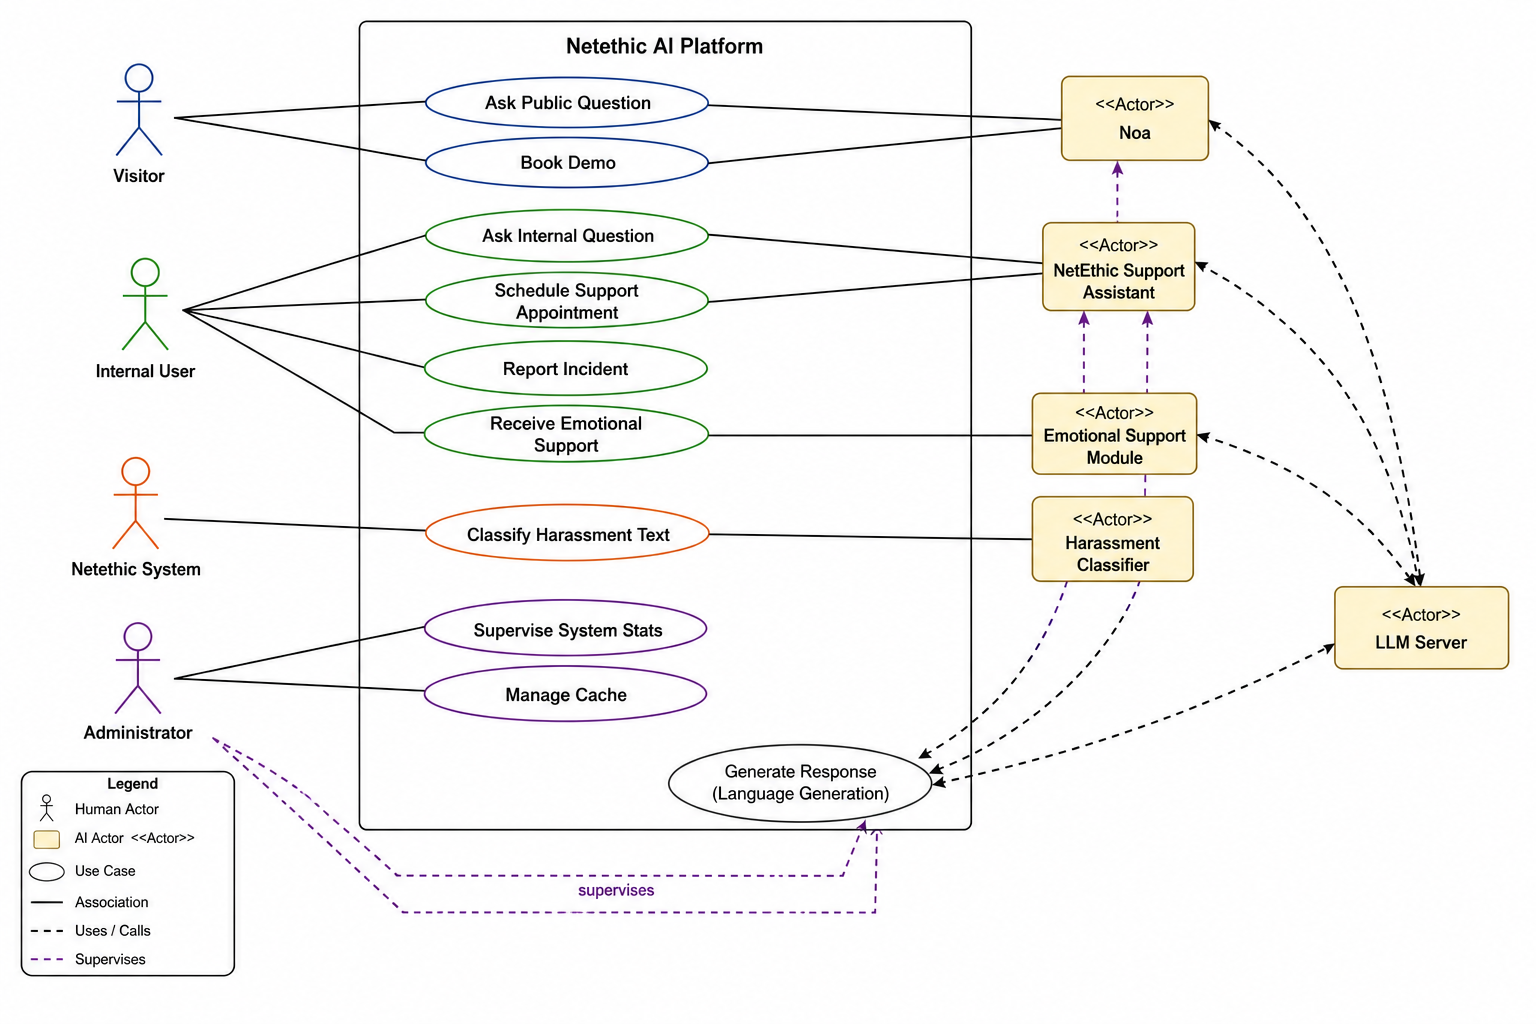
\includegraphics[width=0.95\textwidth]{figures_png/01_use_case_global.png}
\caption{Diagramme de cas d'utilisation global du système}
\label{fig:use_case}
\end{figure}

Le Tableau~\ref{tab:cas_utilisation} décrit les cas d'utilisation essentiels du système.

\vspace{6pt}
\begin{table}[H]
\caption{Description des cas d'utilisation essentiels}
\label{tab:cas_utilisation}
\centering
\small
\setlength{\tabcolsep}{3pt}
\begin{tabular}{|c|p{3cm}|p{2.8cm}|p{7.2cm}|}
\hline
\textbf{ID} & \textbf{Cas d'utilisation} & \textbf{Acteur principal} & \textbf{Description} \\
\hline
CU-01 & Poser une question (site public)
       & Visiteur
       & Le visiteur pose une question en français ou en anglais.
         Noa la traite selon son pipeline : classification, mémoire, recherche, génération. \\
\hline
CU-02 & Réserver une démonstration
       & Visiteur
       & Le visiteur exprime le souhait de planifier une démo.
         L'agent conversationnel collecte son e-mail et son téléphone. \\
\hline
CU-03 & Poser une question (support interne)
       & Utilisateur interne
       & L'utilisateur sélectionne une catégorie parmi les 11~modules, puis pose sa question.
         Le Support Assistant retourne une réponse ancrée dans la documentation. \\
\hline
CU-03b & Consulter les suggestions de questions
        & Utilisateur interne
        & Inclus dans CU-03. L'assistant propose plus de 60~questions prédéfinies réparties
          sur les 11~catégories pour guider l'utilisateur dans l'exploration des fonctionnalités. \\
\hline
CU-04 & Planifier un rendez-vous de support
       & Utilisateur interne
       & Si la documentation ne permet pas de répondre, l'assistant propose un rendez-vous
         et collecte les informations nécessaires. \\
\hline
CU-05 & Signaler un dysfonctionnement
       & Utilisateur interne
       & L'utilisateur déclenche le formulaire de signalement. L'assistant collecte
         les informations et transmet le rapport. \\
\hline
CU-05b & Accéder au portail de support
        & Utilisateur interne
        & Étend CU-04. Lorsqu'aucune documentation ne répond à la question, l'utilisateur
          peut accéder directement au portail de support en ligne pour consulter les
          ressources additionnelles ou contacter l'équipe. \\
\hline
CU-06 & Bénéficier du soutien émotionnel
       & Utilisateur interne
       & Si un signal de détresse est détecté, le module génère une réponse empathique
         et oriente vers le module Accompagnement. En cas d'idéation suicidaire, une alerte est déclenchée. \\
\hline
CU-07 & Classifier un texte
       & Système Netethic
       & La plateforme soumet un texte. Le classificateur retourne les étiquettes détectées,
         le niveau de confiance et un indicateur d'urgence si nécessaire. \\
\hline
CU-08 & Superviser le système
       & Administrateur
       & L'administrateur consulte les statistiques, les rendez-vous collectés,
         les signalements et l'état des caches. \\
\hline
\end{tabular}
\end{table}

% ─────────────────────────────────────────────────────────────────────────────
\section{Identification des besoins techniques}

Cette section décrit l'environnement matériel et logiciel utilisé pour le développement du projet.

\subsection{Environnement de travail}

Le Tableau~\ref{tab:env_travail} présente les équipements et outils utilisés lors du développement.

\vspace{6pt}
\begin{table}[H]
\caption{Environnement de travail}
\label{tab:env_travail}
\centering
\small
\setlength{\tabcolsep}{4pt}
\begin{tabular}{|p{4cm}|p{10.5cm}|}
\hline
\textbf{Composant} & \textbf{Description} \\
\hline
Système d'exploitation & Windows 11 Home (version 10.0.26200) \\
\hline
Environnement de développement & Visual Studio Code avec extensions Python, Scala et Docker \\
\hline
Gestion de version    & Git / GitLab (dépôt : \texttt{gitlab.dataforethic.fr}) \\
\hline
Conteneurisation      & Docker Desktop (Docker Compose v2) \cite{docker} \\
\hline
Gestion de projet     & Méthode Scrum \cite{scrumguide} — réunions hebdomadaires sur Microsoft Teams \\
\hline
Modélisation UML      & Power AMC \\
\hline
\end{tabular}
\end{table}

\subsection{Environnement logiciel}

Le Tableau~\ref{tab:env_logiciel} présente la pile logicielle utilisée.
Les choix technologiques ont été guidés par des critères d'efficacité, d'ouverture
et d'adéquation avec les exigences de chaque module.

\vspace{6pt}
\begin{table}[H]
\caption{Environnement logiciel global}
\label{tab:env_logiciel}
\centering
\small
\setlength{\tabcolsep}{3pt}
\begin{tabular}{|p{2.5cm}|p{4.5cm}|p{1.8cm}|p{5.5cm}|}
\hline
\textbf{Couche} & \textbf{Technologie} & \textbf{Version} & \textbf{Rôle} \\
\hline
Backend Python  & Python               & 3.11             & Langage principal — modules Noa et Support Assistant \\
\hline
Backend Python  & FastAPI \cite{fastapi} & $\geq$ 0.110   & Framework web — expose les interfaces de programmation REST \\
\hline
Backend Scala   & Scala                & 2.12.18          & Langage principal — module classificateur \\
\hline
Backend Scala   & Apache Spark         & 3.5.0            & Moteur de traitement de données à grande échelle \\
\hline
Orchestration   & LangChain \cite{langchain} & $\geq$ 0.2.0 & Orchestration des étapes de traitement conversationnel \\
\hline
Représentation sémantique & sentence-transformers \cite{sbert} & $\geq$ 2.7.0 & Calcul des vecteurs de représentation sémantique \\
\hline
Base documentaire & ChromaDB \cite{chromadb} & $\geq$ 0.5    & Stockage et recherche documentaire par similarité \\
\hline
Serveur LLM     & vLLM — kaisens.fr \cite{vllm2023} & —       & Serveur d'inférence externe, compatible API OpenAI \\
\hline
Modèle LLM      & Mistral-7B-Instruct \cite{mistral2023} & —   & Modèle de génération et de classification de texte \\
\hline
Sessions / Cache & Redis \cite{redis}  & $\geq$ 5.0       & Historique conversationnel et mémoire des réponses \\
\hline
Interface Noa   & React + Vite         & 18 / 5           & Interface chatbot — site public \\
\hline
Interface Support & Streamlit          & $\geq$ 1.32.0    & Interface assistant support interne \\
\hline
Déploiement     & Docker Compose \cite{docker} & —          & Conteneurisation et orchestration des services \\
\hline
\end{tabular}
\end{table}

% ─────────────────────────────────────────────────────────────────────────────
\section{Conclusion}

Ce chapitre a défini les besoins du système dans sa globalité.
Les besoins fonctionnels ont établi les fonctionnalités attendues de chacun des quatre modules.
Les besoins non fonctionnels ont précisé les contraintes de qualité transversales,
notamment en matière de performance, de sécurité, de disponibilité et de conformité RGPD.
Les sept acteurs du système ont été identifiés, avec une représentation particulière
des assistants virtuels et des modules autonomes en tant qu'acteurs à stéréotype \textit{«Actor»}.
Le diagramme de cas d'utilisation a synthétisé l'ensemble de ces interactions.

Dans le chapitre suivant, nous présentons l'état de l'art et les choix technologiques
retenus pour chacun des quatre modules.
